\section*{The Hurewicz Theorem}
\subsection*{Abelianizations}

\begin{proposition}
	The forgetful functor $U : \mathsf{AbGrp} \to \mathsf{Grp}$ admits a left adjoint.
	\label{prop:Ab_grp_abgrp}
\end{proposition}

\begin{proof}
	Let $G \in \ob(\mathsf{Grp})$. For $g,h \in G$, define the \bld{commutator of $g$ and $h$}, written $\sbr[0]{g,h}$, by $\sbr[0]{g,h} := ghg^{-1}h^{-1}$. Moreover, set 
	\begin{equation*}
		X_G := \cbr[0]{\sbr[0]{g,h} : g,h \in G}
	\end{equation*}
	\noindent and define the \bld{commutator subgroup of $G$}, written $\sbr{G,G}$, by $\sbr{G,G} := \langle X_G \rangle$.

	\begin{lemma}
		For all $G \in \ob(\mathsf{Grp})$, $\sbr{G,G} \unlhd G$.
	\end{lemma}

	\begin{proof}
		We follow \cite[265]{lee:topological_manifolds:2011}. Clearly, $\sbr{G,G} \leq G$. By \cite[31]{karpfinger:algebra:2013} we have that 
	\begin{equation*}
		\langle X \rangle = \cbr[0]{x_1 \cdots x_n : n \in \omega \setminus \cbr{0}, x_1,\dots,x_n \in X_G \cup X^{-1}_G}.
	\end{equation*}
	It is easy to check that $X_G = X_G^{-1}$ and thus 
	\begin{equation*}
		\langle X \rangle = \cbr[0]{x_1 \cdots x_n : n \in \omega \setminus \cbr{0}, x_1,\dots,x_n \in X_G}.
	\end{equation*}
	Let $k \in G$ and $x_1 \cdots x_n \in \sbr{G,G}$. Since
	\begin{equation*}
		kx_1 \cdots x_n k^{-1} = kx_1 k^{-1} k x_2 k^{-1} k \cdots k x_n k^{-1}
	\end{equation*}
	\noindent it is enough to show that $k\sbr[0]{g,h}k^{-1} \in \sbr{G,G}$ for all $g,h \in G$. But this immediately follows from
	\begin{equation*}
		k\sbr[0]{g,h}k^{-1} = kghg^{-1}h^{-1}k^{-1} = \sbr[0]{kgk^{-1},khk^{-1}}.
	\end{equation*}
	Thus $\sbr{G,G} \unlhd G$.
	\end{proof}

	\begin{lemma}
		$G \in \ob(\mathsf{AbGrp})$ if and only if $\sbr{G,G} = \cbr{1}$.
		\label{lem:abelian_iff_commutator_trivial}
	\end{lemma}

	\begin{proof}
		Let $G \in \ob(\mathsf{AbGrp})$. Then $\sbr[0]{g,h} = 1$ for all $g,h \in G$, which implies $X_G = \cbr{1}$ and thus $\langle X_G \rangle = \cbr{1}$. Conversly, since $X_G \subseteq \sbr{G,G} = \cbr{1}$, we have that $\sbr[0]{g,h} = 1$ for all $g,h \in G$ which is equivalent to $gh = hg$ for all $g,h \in G$.	
	\end{proof}

	\begin{corollary}
		The quotient group $G/\sbr{G,G}$ is abelian.
	\end{corollary}

	\begin{proof}
		By lemma \ref{lem:abelian_iff_commutator_trivial} it is enough to show that $\sbr[0]{G/\sbr{G,G},G/\sbr{G,G}}$ is trivial. We actually show that $X_{G/\sbr[0]{G,G}} = \cbr{1}$. This immediately follows from
		\begin{equation*}
			\sbr[0]{g\sbr{G,G},h\sbr{G,G}} = ghg^{-1}h^{-1}\sbr{G,G} = \sbr{G,G}
		\end{equation*}
		\noindent for $g\sbr{G,G},h\sbr{G,G} \in G/\sbr{G,G}$.
	\end{proof}

	Hence define $\Ab : \mathsf{Grp} \to \mathsf{AbGrp}$ on objects by
	\begin{equation*}
		\Ab(G) := G/\sbr{G,G}.
	\end{equation*}
	The abelian group $\Ab(G)$ is called the \bld{abelianization of $G$}. On morphisms $\varphi : G \to H$ in $\mathsf{Grp}$ define $\Ab(\varphi) : \Ab(G) \to \Ab(H)$ by setting $\Ab(\varphi)(g\sbr{G,G}) := \varphi(g)\sbr{H,H}$. It is easy to check that this is a well defined morphism of abelian groups.\\
	Let $H \in \ob(\mathsf{AbGrp})$ and $\psi \in \mathsf{AbGrp}(\Ab(G),H)$. Define $\wbar{\psi} \in \mathsf{Grp}(G,U(H))$ by setting $\wbar{\psi}(g) := \psi(g\sbr{G,G})$. If $\varphi \in \mathsf{Grp}(G,U(H))$, define $\wbar{\varphi} \in \mathsf{AbGrp}(\Ab(G),H)$ by $\wbar{\varphi}(g\sbr{G,G}) := \varphi(g)$. It is easy to check that this mapping is actually well defined and that $\wbar{\wbar{\psi}} = \psi$ and $\wbar{\wbar{\varphi}} = \varphi$ holds.
\end{proof}

\begin{exercise}
	In proposition \ref{prop:Ab_grp_abgrp}, check that $\Ab : \mathsf{Grp} \to \mathsf{AbGrp}$ is indeed a functor and the naturality of the bijection in both arguments. 
\end{exercise}

\subsection*{The Hurewicz Morphism}
Since elements of $H_1(X)$ are homology classes of loops, one might suspect that there is a connection between the fundamental group $\pi_1(X,p)$ of a path connected space $X$ at $p$ and the first singular homology group $H_1(X)$. However, since $H_1(X)$ is always abelian and $\pi_1(X,p)$ is not necessarily abelian, they cannot be equal. In this section we use a little trick which makes matters simpler: if $c$ is any singular $n$-chain, not necessarily an $n$-cycle, we can also take its equivalence class modulo $n$-boundaries. We shall denote this class also with $\langle c \rangle$. Clearly, if $c$ is an $n$-cycle, then $\langle c \rangle$ is the usual homology class.

\begin{theorem}[Hurewicz Theorem]
	Let $X \in \ob(\mathsf{Top})$ be path connected and $p \in X$. Then $\Ab(\pi_1(X,p)) \cong H_1(X)$.
	\label{thm:Hurewicz_theorem}
\end{theorem}

\begin{proof}
	We show the result in a sequence of lemmata.
	\begin{lemma}
		The mapping $h : \pi_1(X,p) \to H_1(X)$ defined by $h(\sbr{u}) := \langle u \rangle$ is well defined.
	\end{lemma}

	\begin{proof}
		First of all, since $u \in \Omega(X,p)$, we have that $u \in C_1(X)$. Moreover, $\partial u = u(1) - u(0) = p - p = 0$. Thus $u$ has a homology class $\langle u \rangle$. Let us check that $h$ is well defined. Suppose that $\sbr{u} = \sbr{v}$. Hence $F : u \simeq_{\partial I} v$. Consider the fundamental loop $\omega \in \Omega(\mathbb{S}^1,1)$. By \cite[70]{lee:topological_manifolds:2011}, $\omega$ is a quotient map. Since $u,v \in \Omega(X,p)$, there exist $\wtilde{u},\wtilde{v} \in \mathsf{Top}(\mathbb{S}^1,X)$, such that $\wtilde{u} \circ \omega = u$ and $\wtilde{v} \circ \omega = v$ (see \cite[72]{lee:topological_manifolds:2011}). Since $I$ is a locally compact Hausdorff space \cite[107]{lee:topological_manifolds:2011} implies that $\omega \times \id_I$ is a quotient map. Thus $F$ passes to the quotient and yields a map $\wtilde{F} \in \mathsf{Top}(\mathbb{S}^1 \times I,X)$. Now it is easy to check that $\wtilde{F} : \wtilde{u} \simeq_{\cbr{1}} \wtilde{v}$. Thus an application of the homotopy axiom yields
		\begin{equation*}
			\langle u \rangle = \langle \wtilde{u} \circ \omega \rangle = H_1(\wtilde{u})\langle \omega \rangle = H_1(\wtilde{v})\langle \omega \rangle = \langle \wtilde{v} \circ \omega \rangle = \langle v \rangle.
		\end{equation*}
	\end{proof}

	\begin{lemma}
		Let $u$ be a path in $X$ from $p$ to $q$. Then $\langle \wbar{u}\rangle = - \langle u\rangle$.
		\label{lem:reverse_path_homology}
	\end{lemma}

	\begin{proof}
		From figure \ref{fig:additive_inverse}, we deduce that an appropriate definition of a singular $2$-simplex $\sigma$ would be
		\begin{equation*}
			\sigma(x,y) := u(x).
		\end{equation*}
		Indeed
		\begin{equation*}
			\partial \sigma = \wbar{u} - c_p + u 
		\end{equation*}
		\noindent and since $c_p$ is the boundary of $\sigma_p \in \mathsf{Top}(\Delta^2,X)$ defined by $\sigma_p(x,y) := p$, we have that $\wbar{u} + u$ is a boundary.
		\begin{figure}[h!tb]
			\centering
			\begin{subfigure}[b]{.4\textwidth}
				\centering
				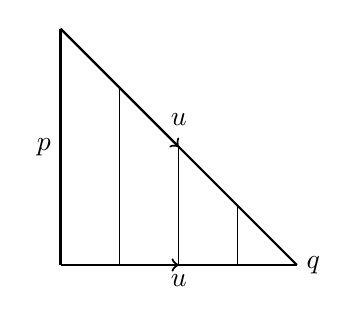
\begin{tikzpicture}[scale = 3]
					\draw [thick] (0,0) -- (1,0);
					\draw [thick] (0,0) -- (0,1);
					\draw [thick] (0,1) -- (1,0);
					\draw [thick,->] (0,0) -- (.5,0);
					\draw [thick,->] (0,1) -- (.5,.5);
				
					\draw [thin] (.25,0) -- (.25,.75);
					\draw [thin] (.5,0) -- (.5,.5);
					\draw [thin] (.75,0) -- (.75,.25);

					\draw (.5,0) node[below] {$u$};
					\draw (.5,.55) node[above] {$u$};
					\draw (0,.5) node[left] {$p$};
					\draw (1,0) node[right] {$q$};
				\end{tikzpicture}
				\caption{$\langle \wbar{u} \rangle = - \langle u \rangle$.}
				\label{fig:additive_inverse}
			\end{subfigure}
			~
			\begin{subfigure}[b]{.4\textwidth}
				\centering
				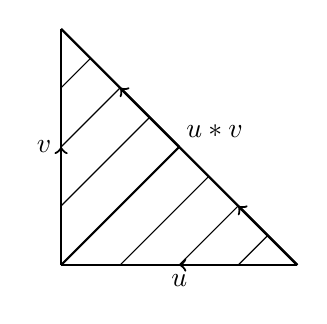
\begin{tikzpicture}[scale = 3]
					\draw [thick] (0,0) -- (1,0);
					\draw [thick] (0,0) -- (0,1);
					\draw [thick] (0,1) -- (1,0);
					\draw [thick] (0,0) -- (.5,.5);
					\draw [thick,->] (1,0) -- (.75,.25);
					\draw [thick,->] (.5,.5) -- (.25,.75);
					\draw [thick,->] (1,0) -- (.5,0);
					\draw [thick,->] (0,0) -- (0,.5);
				
					\draw [thin] (.25,0) -- (.625,.375);
					\draw [thin] (.5,0) -- (.75,.25);
					\draw [thin] (.75,0) -- (.875,.125);

					\draw [thin] (0,.25) -- (.375,.625);
					\draw [thin] (0,.5) -- (.25,.75);
					\draw [thin] (0,.75) -- (.125,.875);

					\draw (.5,0) node[below] {$u$};
					\draw (.65,.5) node[above] {$u \ast v$};
					\draw (0,.5) node[left] {$v$};
				\end{tikzpicture}
				\caption{$\langle u \ast v \rangle = \langle u \rangle + \langle v \rangle$.}
				\label{fig:hurewicz_homomorphism}
			\end{subfigure}
		\end{figure}
	\end{proof}

	\begin{lemma}
		\label{lem:concatenation_addition}
		Let $u$ and $v$ be paths in $X$ from $p$ to $q$ and from $q$ to $r$, respectively. Then $\langle u \ast v \rangle = \langle u \rangle + \langle v \rangle$.	
	\end{lemma}

	\begin{proof}
		Consider figure \ref{fig:hurewicz_homomorphism}. The thin lines correspond to where $y - x$ is constant. Hence define $\sigma : \Delta^2 \to X$ by
		\begin{equation*}
			\sigma(x,y) := \ccases{
				u(y - x + 1) & 0 \leq y \leq x \leq 1,\\
				v(y - x) & 0 \leq x \leq y \leq 1.
			}
		\end{equation*}
		An application of the gluing lemma shows that $\sigma$ is actually a singular $2$-simplex. Moreover
		\begin{equation*}
			\partial \sigma = u \ast v - v + \wbar{u}.
		\end{equation*}
		Hence lemma \ref{lem:reverse_path_homology} yield
		\begin{equation*}
			0 = \langle u \ast v - v + \wbar{u}\rangle = \langle u \ast v \rangle - \langle v \rangle - \langle u \rangle.
		\end{equation*}
	\end{proof}

	\begin{corollary}
		\label{cor:h_homomorphism}
		$h$ is a morphism of groups.
	\end{corollary}

	\begin{corollary}
		\label{cor:composable_associative_homology}
		Let $u,v,w$ be composable paths in $X$. Then $\langle (u \ast v) \ast w \rangle = \langle u \ast (v \ast w) \rangle$.
	\end{corollary}

	\begin{lemma}
		$h$ is surjective.
	\end{lemma}

	\begin{proof}
		Let $x \in X$. If $x = p$, define $\gamma_p := c_p$. If $x \neq p$, by the path connectedness of $X$ we can choose a path $\gamma_x$ from $p$ to $x$. Hence we get a map $\gamma : X \to \mathsf{Top}(\Delta^1,X)$. Extending by linearity yields a mapping $\gamma : C_0(X) \to C_1(X)$. Let $c := \sum_{k = 1}^n m_k \sigma_k$ be a $1$-cycle in $X$. Consider
		\begin{equation*}
			\sbr{u} := \sbr[0]{\gamma_{\sigma_1(0)} \ast \sigma_1 \ast \overline{\gamma_{\sigma_1(1)}}}^{m_1} \cdots \sbr[0]{\gamma_{\sigma_n(0)} \ast \sigma_n \ast \overline{\gamma_{\sigma_n(1)}}}^{m_n} \in \pi_1(X,p). 
		\end{equation*}
		Now lemma \ref{lem:reverse_path_homology} and \ref{lem:concatenation_addition}, corollary \ref{cor:h_homomorphism} and \ref{cor:composable_associative_homology} yields
		\begin{align*}
			h(\sbr{u}) &= \sum_{k = 1}^n m_k \langle\gamma_{\sigma_k(0)} \ast \sigma_k \ast \overline{\gamma_{\sigma_k(1)}}\rangle\\
			&= \sum_{k = 1}^n m_k \del[1]{\langle\gamma_{\sigma_k(0)}\rangle + \langle\sigma_k\rangle + \langle \overline{\gamma_{\sigma_k(1)}}\rangle}\\
			&= \sum_{k = 1}^n m_k \del[1]{\langle\gamma_{\sigma_k(0)}\rangle + \langle\sigma_k\rangle - \langle \gamma_{\sigma_k(1)}}\rangle\\
			&= \langle c \rangle - \sum_{k = 1}^n m_k \langle \gamma_{\sigma_k(1) - \sigma_k(0)}\rangle\\
			&= \langle c \rangle - \sum_{k = 1}^n m_k \langle \gamma_{\partial \sigma_k}\rangle\\
			&= \langle c \rangle - \langle \gamma_{\partial c}\rangle\\
			&= \langle c \rangle.
		\end{align*}
	\end{proof}

	Lastly, we want to show that $\ker h = \sbr[0]{\pi_1(X,p),\pi_1(X,p)}$. Since then the first isomorphism theorem implies $\Ab(\pi_1(X,p)) \cong H_1(X)$. Since $H_1(X)$ is abelian, clearly $\sbr[0]{\pi_1(X,p),\pi_1(X,p)} \subseteq \ker h$ and thus $h$ factors uniquely $\wtilde{h} : \Ab(\pi_1(X,p)) \to H_1(X)$. The next lemma will be useful.
	
	\begin{lemma}
		\label{lem:nullhomotopic_loop}
		Let $\sigma : \Delta^2 \to X$ be a singular $2$-simplex. Define $\sigma^{(k)} := \sigma \circ \varphi^2_k$ for $k = 0,1,2$. Then $\sbr[0]{\sigma^{(0)} \ast \overline{\sigma^{(1)}} \ast \sigma^{(2)}} = \sbr[0]{c_{\sigma(e_1)}}$.
	\end{lemma}

	\begin{proof}
		Let $u := \sigma^{(0)} \ast \overline{\sigma^{(1)}} \ast \sigma^{(2)}$. Since $\mathbb{B}^2 \approx \Delta^2$, we can consider $\sigma : \mathbb{B}^2 \to X$. One can check that the circle representative $\wtilde{u}$ of $u$ is the reparametrized restriction $\sigma \vert_{\mathbb{S}^1}$. Since reparametrizations are invariant under homotopies, we have that $u$ is a nullhomotopic loop.
	\end{proof}

	Let $\sigma \in \mathsf{Top}(\Delta^1,X)$. Define $g(\sigma) := \sbr[0]{\gamma_{\sigma(0)} \ast \sigma \ast \overline{\gamma_{\sigma(1)}}}_{\Ab}$, where $\sbr{u}_{\Ab}$ denotes the equivalence class of $\sbr{u}$ in $\Ab(\pi_1(X,p))$. Since $\Ab(\pi_1(X,p))$ is abelian, extension by linearity yields a map $g : C_1(X) \to \Ab(\pi_1(X,p))$.

	\begin{lemma}
		\label{lem:g_vanishes_on_boundaries}
		$g$ vanishes on $\im \partial_2$.	
	\end{lemma}

	\begin{proof}
		Let $\sigma \in \mathsf{Top}(\Delta^2,X)$. Then lemma \ref{lem:nullhomotopic_loop} yields
		\begin{align*}
			g(\partial \sigma) &= g\del[1]{\sigma^{(0)}} g\del[1]{\sigma^{(1)}}^{-1}g\del[1]{\sigma^{(2)}}\\
			&= \sbr[1]{\gamma_{\sigma(e_1)} \ast \sigma^{(0)} \ast \overline{\gamma_{\sigma(e_2)}} \ast \gamma_{\sigma(e_2)} \ast \overline{\sigma^{(1)}} \ast \overline{\gamma_{\sigma(e_0)}} \ast \gamma_{\sigma(e_0)} \ast \sigma^{(2)} \ast \overline{\gamma_{\sigma(e_1)}}}_{\Ab}\\
			&= \sbr[1]{\gamma_{\sigma(e_1)} \ast \sigma^{(0)} \ast \overline{\sigma^{(1)}} \ast \sigma^{(2)} \ast \overline{\gamma_{\sigma(e_1)}}}_{\Ab}\\
			&= \sbr[1]{\gamma_{\sigma(e_1)} \ast c_{\sigma(e_1)} \ast \overline{\gamma_{\sigma(e_1)}}}_{\Ab}\\
			&= \sbr{c_p}_{\Ab}.
		\end{align*}
	\end{proof}

	By lemma \ref{lem:g_vanishes_on_boundaries}, $g$ passes to the quotient and yields a map $\wtilde{g} : H_1(X) \to \Ab(\pi_1(X,p))$. Moreover
	\begin{equation*}
		(\wtilde{g} \circ \wtilde{h})\sbr{u}_{\Ab} = \wtilde{g}\del[1]{h\sbr{u}} = \wtilde{g}\langle u \rangle = g(u) = \sbr[0]{c_p \ast u \ast \overline{c_p}}_{\Ab} = \sbr{u}_{\Ab}
	\end{equation*}
	\noindent and thus $\wtilde{h}$ admits a retraction in $\mathsf{AbGrp}$ which implies that $\wtilde{h}$ is injective. Hence $\ker \wtilde{h}$ is trivial and thus if we write $\pi : \pi_1(X,p) \to \Ab(\pi_1(X,p))$ for the canoncial projection
	\begin{equation*}
		\ker h = \ker(\wtilde{h} \circ \pi) = (\wtilde{h} \circ \pi)^{-1}(0) = \pi^{-1}\del[1]{\wtilde{h}^{-1}(0)} = \pi^{-1}(0) = \sbr[0]{\pi_1(X,p),\pi_1(X,p)}. 
	\end{equation*}	
\end{proof}

\begin{definition}[Hurewicz Homomorphism]
	Let $X \in \ob(\mathsf{Top})$ and $p \in X$. The homomorphism $h : \pi_1(X,p) \to H_1(X)$ defined in theorem \ref{thm:Hurewicz_theorem} is called the \bld{Hurewicz homomorphism}.
\end{definition}

\begin{proposition}
	Let $U : \mathsf{AbGrp} \to \mathsf{Grp}$ denote the forgetful functor. Then the Hurewicz homomorphism is a natural transformation $\pi_1 \Rightarrow U \circ H_1$.
\end{proposition}

\begin{proof}
	
\end{proof}

